\section{Shape index and query-shape containment}

We define a shape index as a set of mappings between RDF data shapes and sets of resources.
Additionally, an SI has an associated domain (set of URLs)
and a flag indicating if the SI is \emph{complete}.
A SI is complete when every resource in the domain is associated with a shape.
In a SI when a shape is in relation to a set of RDF resources then the shape \emph{must} validate those resources.
Furthermore, every set of triples respecting the shape in the domain \emph{must} be located inside one resource of the set.

Our approach consists of determining before the traversal of a whole domain the location of the useful resources for the query execution.
This data discovery operation results in the implicit pruning of links leading to surely non-contributing resources.
In this approach, the query engine can start its processing with a permissive reachability criteria
such as $c_{all}$ \cite{Hartig2012} or the Solid state of the art reachability criterion ($\mathrm{c_{LDP}}$ and $\mathrm{c_{type-index}}$) \cite{Taelman2023}
and not suffer from the associated longer execution time during the traversal of environments containing a SI.
After the analysis of the SI with the query provided by the user the criteria can be adapted to become more restrictive within the domain of the SI.
For that purpose, the query engine must first discover the SI in the current (sub)domain.
In the case of Solid, the SI should be at the root of the pod to be easily discoverable.
The approach is schematized at Figure \ref{fig:shape_index}.
Source selection with an SI consists of interpreting the binding results from a \emph{query-shape containment} problem similar to the classic query containment problem \cite{afariQCE, Spasi2023}.
To perform this algorithm, we transform the shapes into queries ($Q_{s}$) \cite{labragayo2017validating, Delva2021}.
The algorithm divides the query from the user into multiple star patterns with their dependencies ($Q_{star}$).
Then it pushdown \cite{Yang2021FlexPushdownDBHP} the (sub)queries to the level of source selection to evaluate if the $Q_{star}$ are contained inside the $Q_s$ of the SI.
If all the $Q_{star}$ are contained in a $Q_{s}$ or have no binding with any $Q_{s}$
the reachability criteria is adapted to ignore all the resources not linked to a $Q_{s}$ even if the SI is \emph{incomplete}.
If the SI is \emph{complete} and not all the $Q_{star}$ are contained in a $Q_{s}$ the reachability criteria can be adapted
to visit every resource in relation to a $Q_{s}$ with a partial binding with a $Q_{star}$.
In a similar case with a \emph{incomplete} SI the query engine can only use the SI for data discovery.
This case is similar to the usage of the type index but with a more reaching ability to match a query with the index 
because shapes in their definition describe the properties (RDF predicates) of the entities whereas the type index only provides the classes IRIs.
It would be possible to dereference the class IRIs to get information about the properties (if available) however it is not the current practice \cite{Taelman2023}.
A comparison of the RDF data shapes and RDF class approach due to their potential similarities is delegated to future works.
It has to be noted that in the literature \cite{demeester_swj_2021} there are comparisons 
between the two approaches in the context of data validation but it is left to be determined if their frame of comparison is compatible with our current problem
and foreseen opportunities.

\begin{figure}
    \centering
    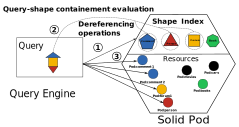
\includegraphics[width=0.5\textwidth]{figure/shape_containement}
    \caption{A schema of the source selection algorithm with a SI. First, the SI is dereference, 
    then the \emph{query-shape containment} is performed and lastly only the relevant resources are dereferenced.}
    \label{fig:shape_index}
\end{figure}